\definecolor{bblue}{HTML}{4F81BD}
\definecolor{rred}{HTML}{C0504D}
\definecolor{ggreen}{HTML}{9BBB59}
\definecolor{ppurple}{HTML}{9F4C7C}
\definecolor{yyellow}{HTML}{CCAA40}
\definecolor{bbrown}{HTML}{662233}
\definecolor{excelGreen}{HTML}{50AA45}
\definecolor{sibPurple}{HTML}{822689}

\newcommand{\mycbox}[1]{\tikz{\path[draw=#1,fill=#1] (0,0) rectangle (0.3cm,0.3cm);}}

\chapter{Evaluation}

\paragraph{} This chapter shall discuss the effectiveness of the Excello implementation with regards to the success criteria and by showcasing examples. The conversion of an existing MIDI corpus to the Excello notation using the converter from MIDI will demonstrate the expressiveness of the notation. Next I shall explain the summative evaluation and use the data from this to assess the features implemented in the participatory design process and to reason about Excello using the CDN framework \cite{blackwell:tutorial}. Finally, the ethics and data handling procedures shall be covered.

\section{Excello Success}

\paragraph{} Both a notation for music expression and a program integrated into Excel for the playback of this expression has been implemented. As required by the success criteria, users can play multiple notes and chords of different durations. These can be combined into looped sequences with a defined tempo. In the participatory design process additional features were added as extensions. Defining multiple successive notes in a cell, turtles calculating how far they should move and nested instructions with repeats are additional features facilitating more efficient notation. Custom Excel functions, a chord adding tool and faster turtle toggling allows users to work more efficiently. Figure \ref{evaluation:excelloFranzRedacted} shows Excello in use with participant's arrangement.

\begin{figure}[tbh]
\centerline{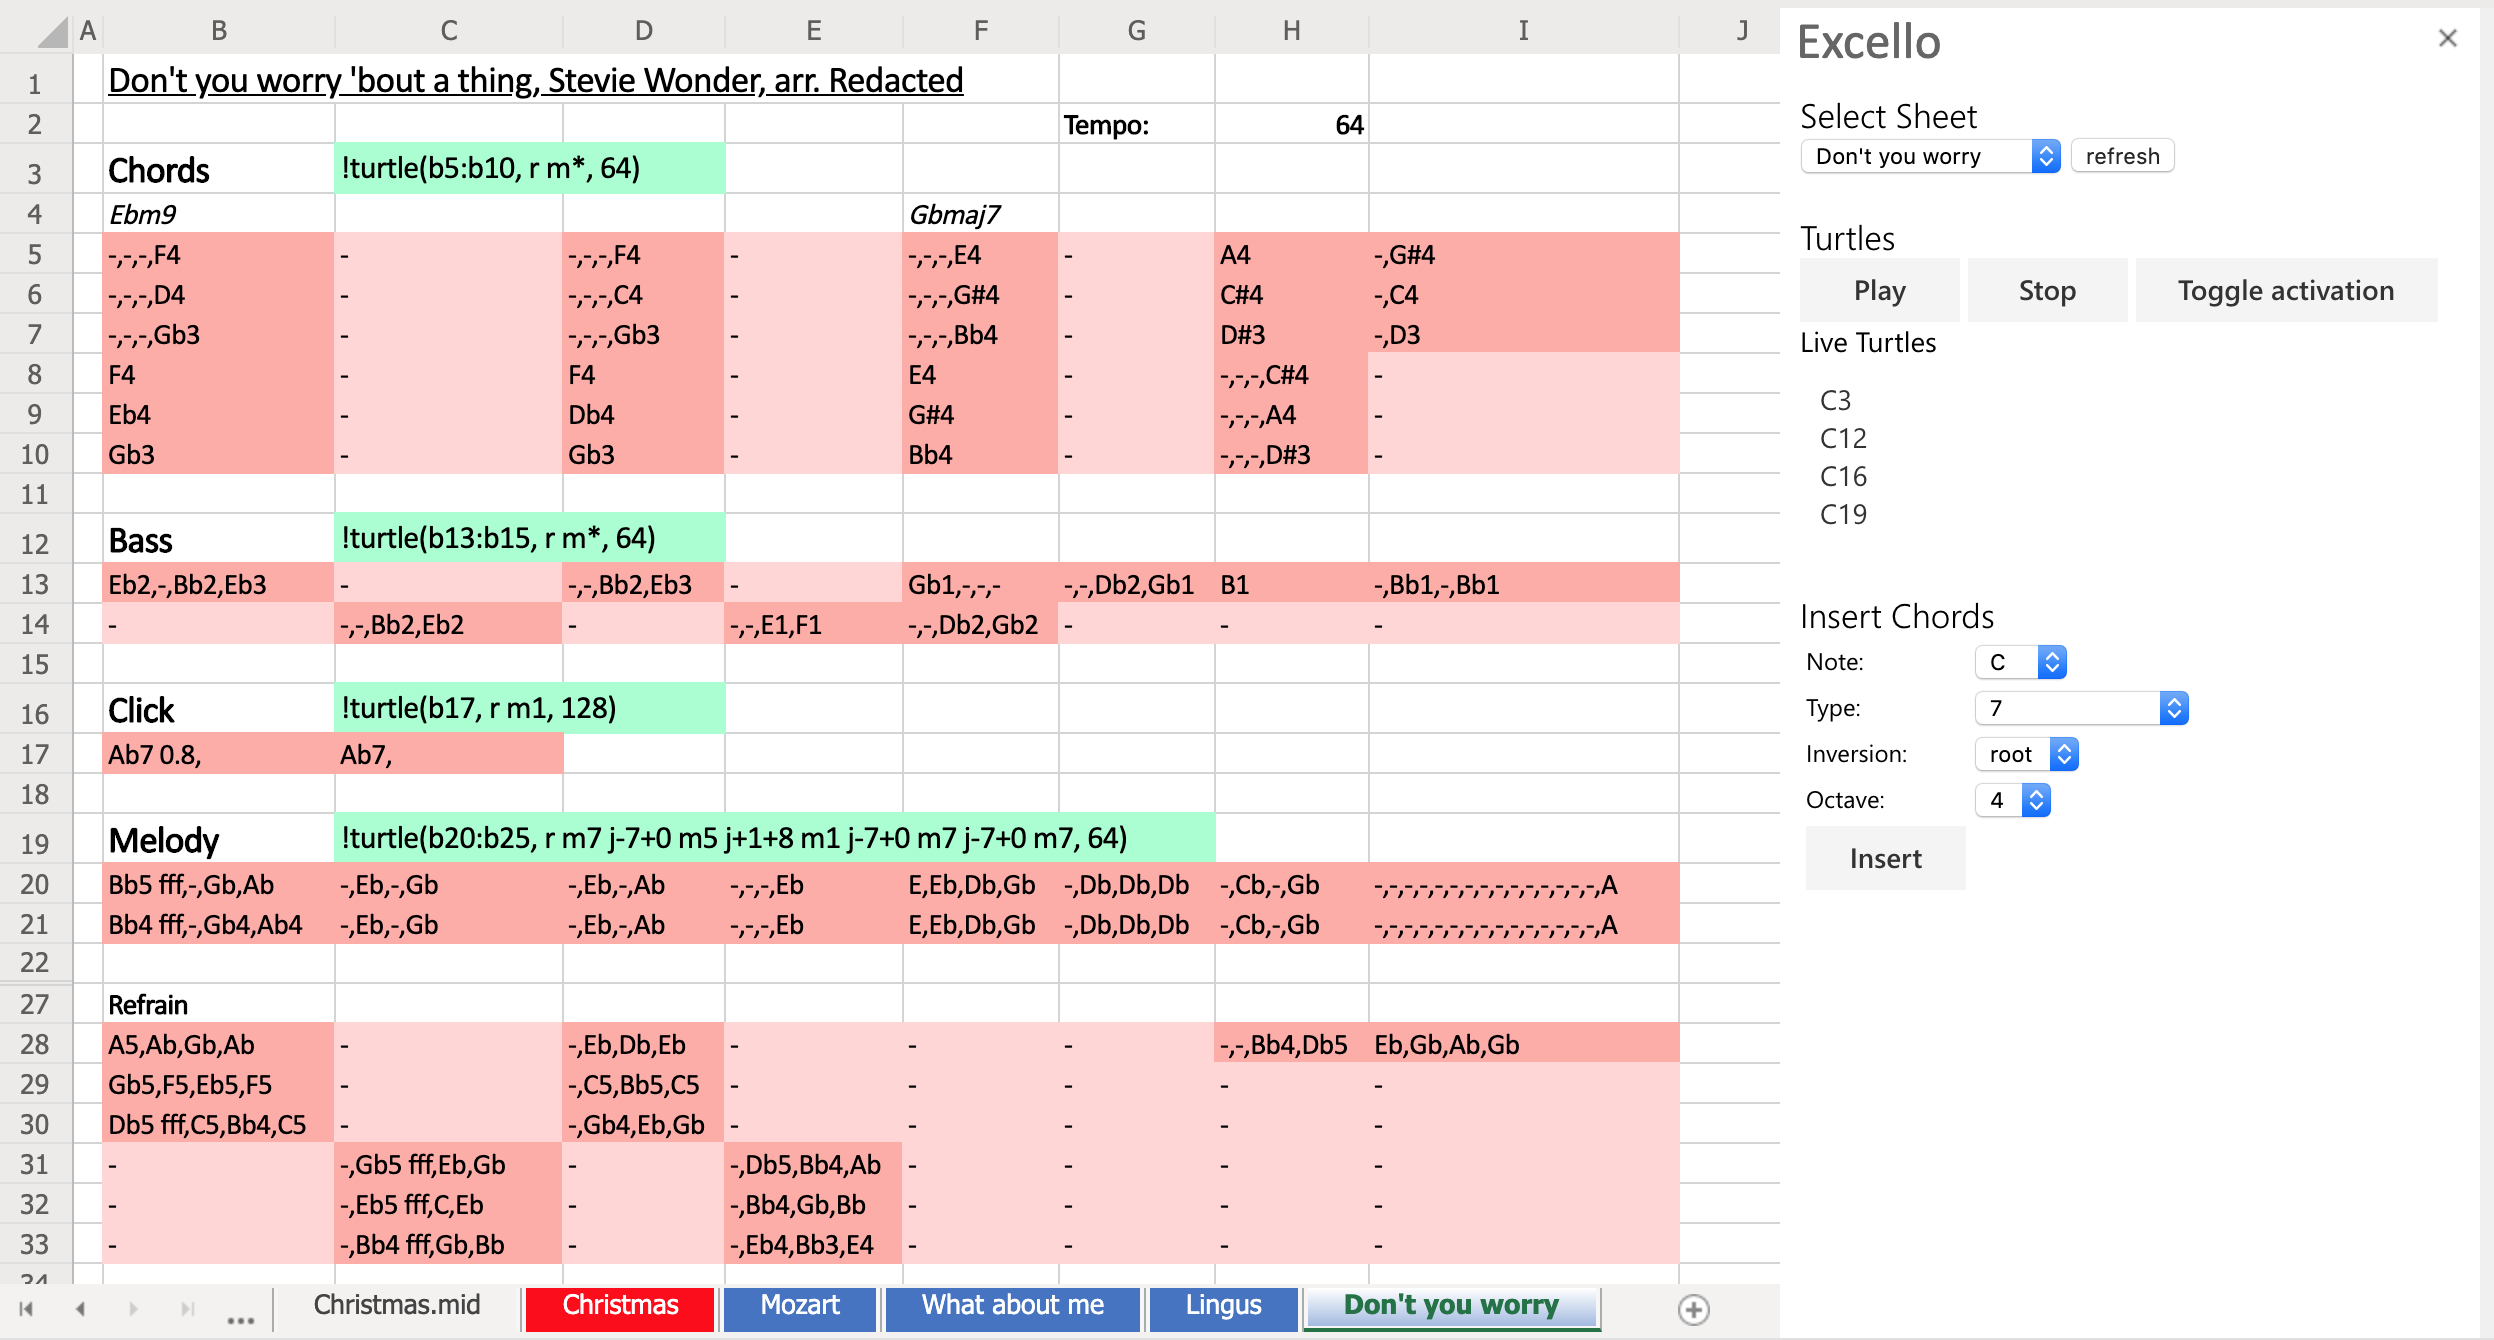
\includegraphics[width=150mm]{figs/excelloFranzRedacted.png}}
\caption{An arrangement with separated and labelled parts per instrument. Turtles refer to a global tempo at the top of the spreadsheet.}
\label{evaluation:excelloFranzRedacted}
\end{figure}

\paragraph{} The first section of Piano Phase by Steve Reich consists of two equal piano melodies, one slightly faster than the other. The two parts move out of phase before aligning at different offsets. This is included as an example for many end-user programming tools. This is implemented in Manhattan using three rows of 24 columns \cite{nash:manhattan}. Sonic Pi defined the notes in one line and eight additional lines are required for playback. Piano Phase can not be concisely notated by western staff notation. Excello only requires two cells to define two turtles of different speeds in addition to the notes. All three implementations are shown in figure \ref{evaluation:phase}.

% \begin{figure}[tbh]
% \centerline{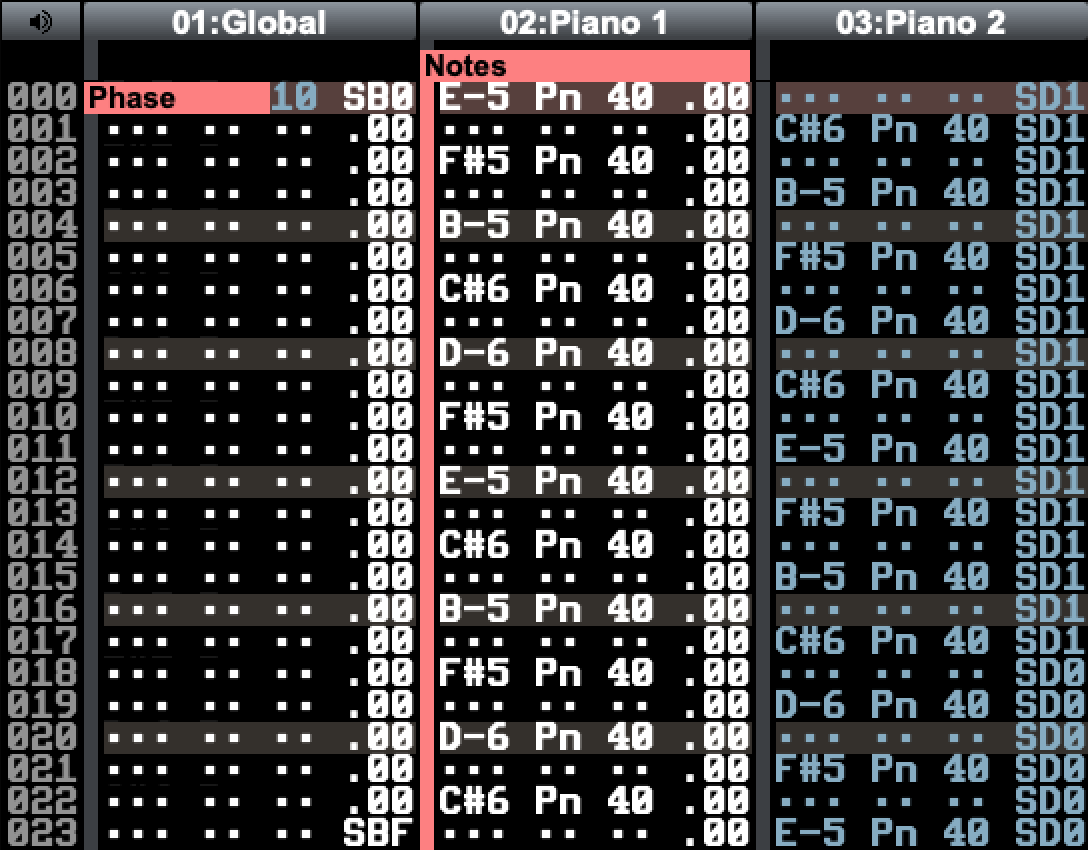
\includegraphics[width=150mm]{figs/manhattanPhase.png}}
% \caption{Piano Phase defined in Manhattan. Column 01 keeps track of the phase, 02 defines the notes and 03 is the phased notes - defined with formulae than update depending on the phase and defined notes.}
% \label{evaluation:manhattanPhase}
% \end{figure}

% \begin{figure}[tbh]
% \centerline{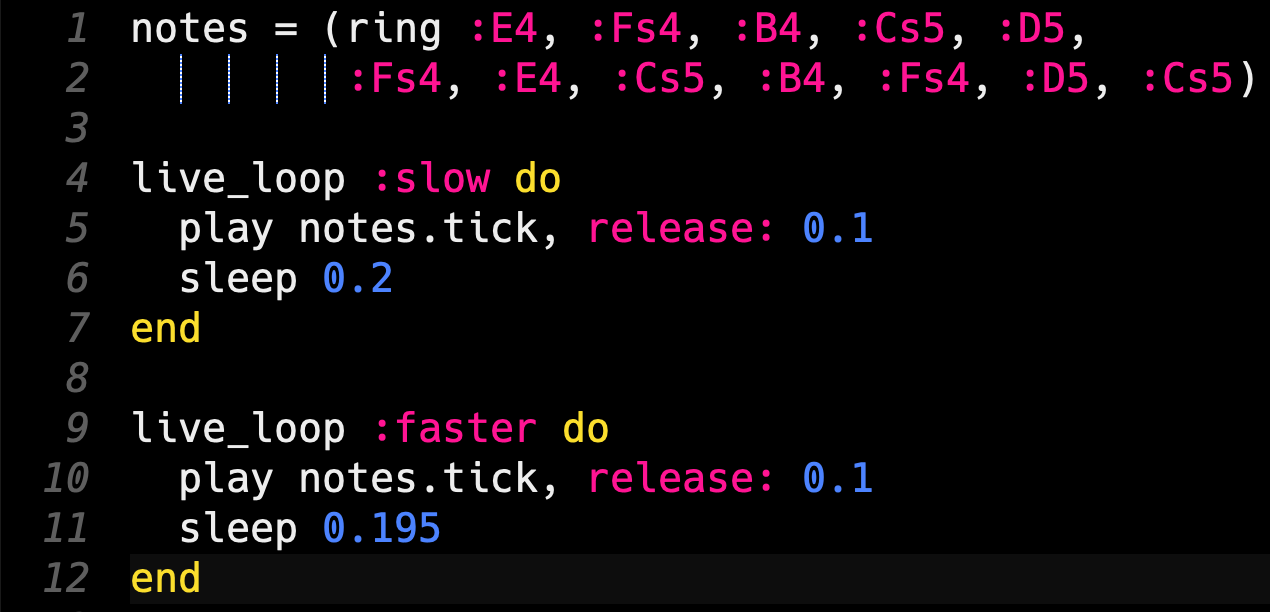
\includegraphics[width=150mm]{figs/sonicPiPhase.png}}
% \caption{XXXX}
% \label{evaluation:sonicPiPhase}
% \end{figure}

% \begin{figure}[tbh]
% \centerline{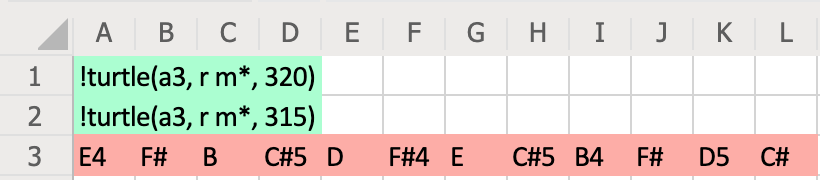
\includegraphics[width=150mm]{figs/excelloPhase.png}}
% \caption{XXXX}
% \label{evaluation:excelloPhase}
% \end{figure}

\begin{figure}[ht]
\begin{tabular}{cc}
  \multirow{3}{*}[2.72cm]{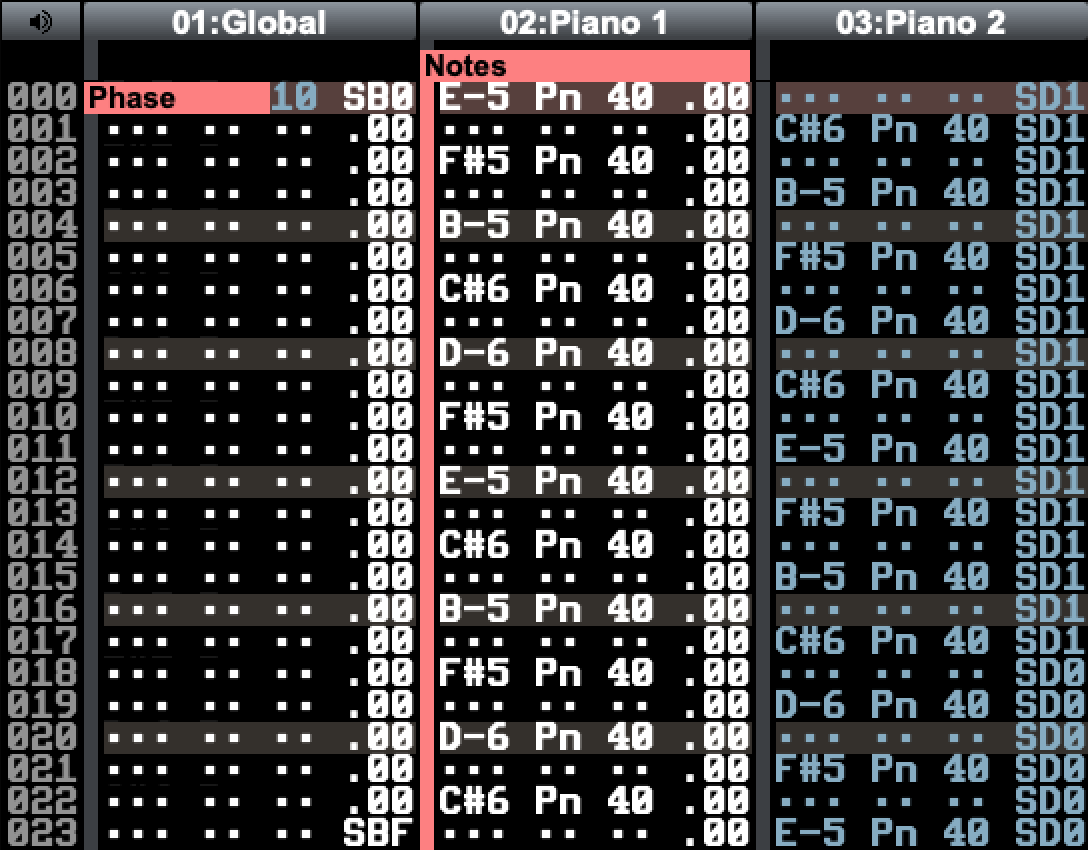
\includegraphics[width=65mm]{figs/manhattanPhase.png}} & 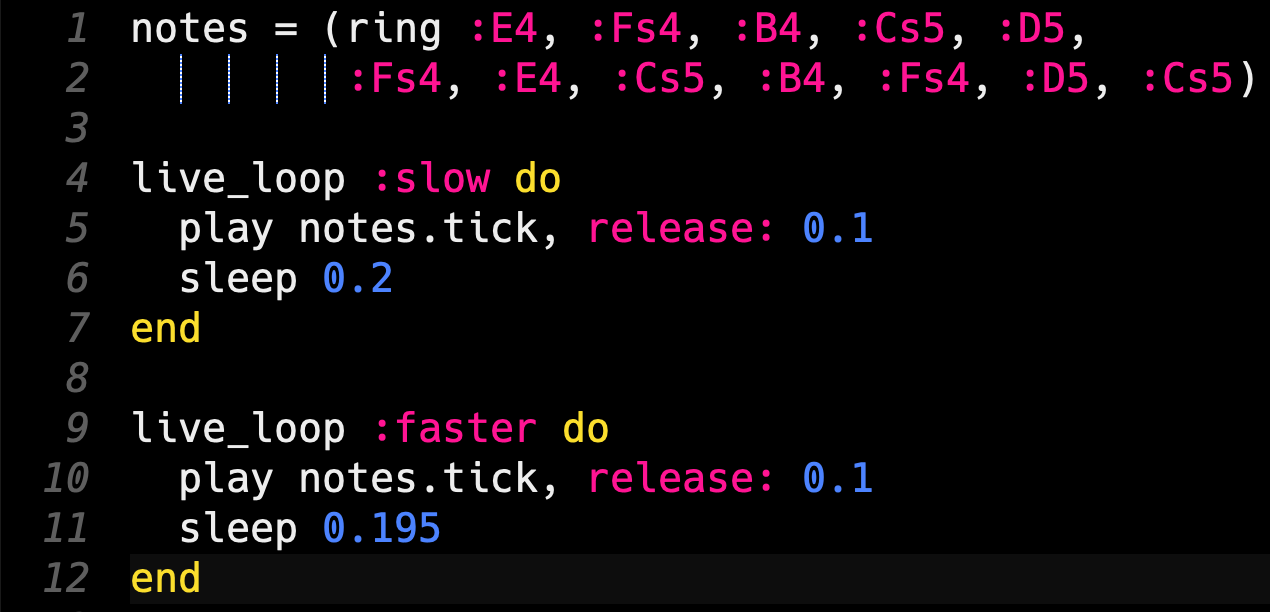
\includegraphics[width=65mm]{figs/sonicPiPhase.png} \\
  & (b) The defined notes are played\\
  & by two concurrent loops with\\
  & different gaps between each note.\\[6pt]
  (a) Column 01 keeps track of the phase,& \multirow{2}{*}{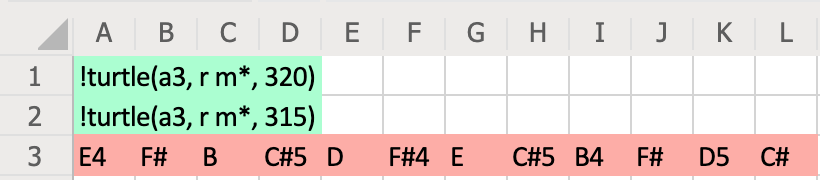
\includegraphics[width=65mm]{figs/excelloPhase.png}} \\
  02 defines the notes and 03 is the &\\
  phased notes - defined with formulae &\\
  that update depending on the phase and& (c) Two turtles play the same\\
  defined notes.& notes at different speeds.\\
\end{tabular}
\caption{Implementations of Steve Reich's Piano Phase in a) Manhattan, b) Sonic Pi, c) Excello}
\label{evaluation:phase}
\end{figure}

\section{MIDI Corpus Conversion}

\paragraph{} Whilst being able concisely notate music western notation and other end-user programming systems do not facilitate, Excello can exactly express any combination of concurrent note onset and offsets. Therefore any piece defined in MIDI can be expressed in Excello. In MIDI allows tempo can be redefined within a track, this is not be accounted for. If instead the time between note onsets and offsets is adjusted, the uncompressed file will account for this but compressing algorithm will fail as the difference between notes may become a non-integer multiple of the minimum. Instrument specific effects such as piano pedals are not supported. This naive conversion can result in unwieldy spreadsheet sizes. One conversion method compresses the representation by dividing the difference between notes by the minimum difference in not onset between any two notes. Provided the difference between any two notes is a multiple of the minimum difference, this compression method is lossless, whilst resulting in spreadsheets using orders of magnitude fewer cells. Therefore this method would not accurately convert quavers against triplets (three notes played in the same time as two) provided these notes were not multiples of a smaller note. Given the lengths of MIDI notes can be different to the time the note occupies in notation, to automate the compression, an assumption on the ratio of note lengths was required. The modal compression algorithm is lossy if the minimum note distance is not the modal distance. This is useful if there are ornaments or note within a piece that dramatically decrease the minimum distance but occur infrequently. Therefore their loss may be tolerable for a more efficient representation.

\paragraph{} I have converted three MIDI corpora. The first is a collection of 497 Bach chorales\footnote{Accessed from https://github.com/jamesrobertlloyd/infinite-bach/tree/master/data/chorales/midi} made by Margaret Greentree. The second is 277 piano pieces\footnote{http://piano-midi.de/midis.htm} help by Bernd Krueger  under a creative commons license. Finally 194 Bach pieces made available from "A Johann Sebastian Bach Midi Page"\footnote{http://www.bachcentral.com/midiindex.html}. This is not all the files available from this site as some were not readable by the python MIDI reader. All 968 MIDI files were converted using all three methods.

\paragraph{} The language of Excello is expressive enough to represent MIDI files and can do so concisely provided the condition of minimum note onset differences is maintained.

\section{Summative Evaluation Sessions}

\paragraph{} Of the 21 users who participated in formative evaluation, 19 had continued using Excello. These users all filled out a summative evaluation questionnaire. First a review of the features that had been added since the initial sessions was given. To ensure users had a sufficient understanding of the interface before giving feedback, a short transcription task involving some original composition by the users was given.

\paragraph{} The questionnaire first assessed the success of the features added during the participatory design process by comparing the interface before and after a feature had been added. Seven-point Likert scale questions were given to test if the issues had been solved and if overall the change rendered the system more preferable. The remaining questions were based on Blackwell and Green's CDN questionnaire \cite{blackwell:questionnaire}. CDNs can be used to analyse musical notation \cite{blackwell:notation} in addition to software systems \cite{green:cdn}, therefore it is a suitable tool for the discussion of the Excello notation and interface. Because dimensions have different significances for the different activities \cite{blackwell:tutorial}, users identified what percentage of their time they spent carrying out the five different user activities (searching for information, translating, incrementation, modification and exploratory design). Likert scale questions focusing on closeness of mapping, consistency, secondary notation, viscosity and visibility were used as planned in the project proposal. It was suspected that reasoning about cognitive dimensions would be more challenging for participants, so to reduce the expected variance, only a five-point Lichard scale was used. Usage and CDN questions were also answered with respect to the user's preferred interface for music manipulation, composition or transcription. 12 users chose Sibelius, which shall be used for comparison.

\section{Success of Participatory Design}

\paragraph{} For each feature added, Excello with this feature (system 2) was compared to first prototype implementation. The following charts show the frequency of Likart scale responses for each question. I considered the mode of the Likert scale \cite{barry:likert}. A Chi-Squared goodness-of-fit test tests if the distribution is significantly different to uniform. As all expected values must be greater than 1 and 80\% greater than or equal to five \cite{ross:introductory} and the expected frequency for one result is $19/7 \approx 2.7$, I combine Strongly Disagree with Disagree, Strong Agree with Agree and the remaining three options into a third group. The p-value given is from the Chi-Squared test using these three categories.

\subsection{Dynamics in the Cell}

\begin{table}[!htbp]
\centering
% \caption{Grammar rules for turtle movement instructions. $z \in \mathbb{Z}, n \in \mathbb{N}, c \in \texttt{[A-Za-z]}^{+}$.}
\vspace{1pt}
\begin{tabular}{|l|l|l|} \hline
\textbf{Statement}&\textbf{Mode}&\textbf{p-value}\\ \hline
\mycbox{bblue} It is easier to figure out the turtles path&Strongly Agree&0.0000\\ \hline
\mycbox{rred} It is easier to figure out what dynamics different&Strongly Agree&0.0146\\
notes are played at&&\\ \hline
\mycbox{ggreen} It is easier to tell the order in which dynamics are applied&Strongly Agree&0.0000\\ \hline
\mycbox{ppurple} It is easier to write dynamics in the correct place&Strongly Agree&0.0000\\ \hline
\mycbox{yyellow} Overall system 2 is preferable&Strongly Agree&0.0000 \\ \hline
\end{tabular}
\label{evaluation:cellDynamics}
\end{table}

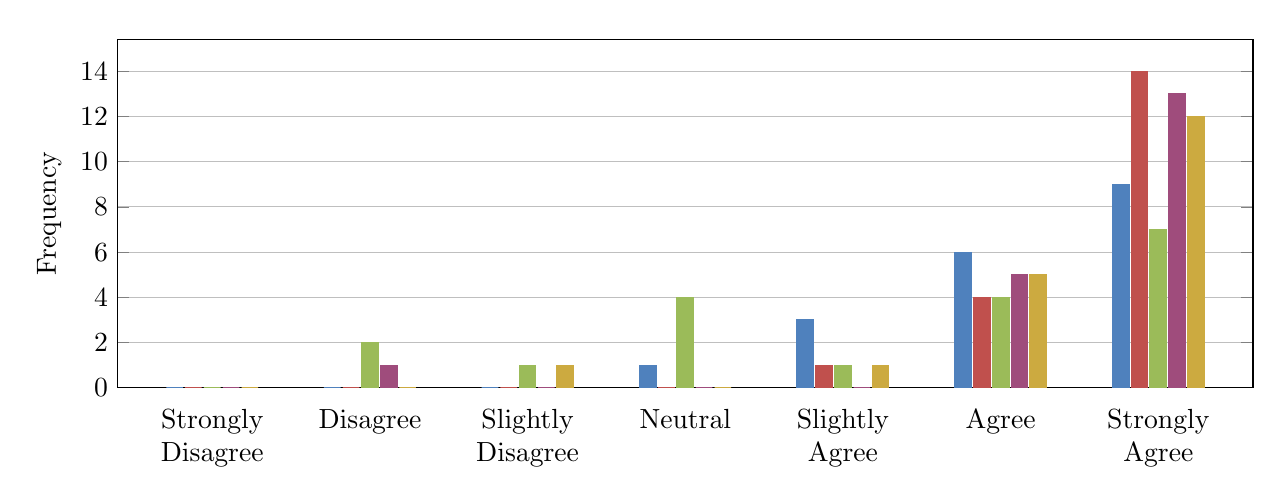
\begin{tikzpicture}
    \begin{axis}[
      % width  = \textwidth,
      width = 16cm,
      height = 6cm,
      major x tick style = transparent,
      ybar=2*\pgflinewidth,
      bar width=6pt,
      ymajorgrids = true,
      ylabel = {Frequency},
      %xlabel = {Likert Scale Result},
      symbolic x coords= {-3,-2,-1,0,1,2,3},
      xticklabels = {Strongly Disagree,Disagree,Slightly Disagree,Neutral,Slightly Agree,Agree,Strongly Agree},
      xtick = data,
      ytick = {0,2,4,6,8,10,12,14},
      x tick label style  = {text width=2cm,align=center},
      scaled y ticks = false,
      % enlarge x limits=0.25,
      ymin=0,
      legend cell align=left,
      legend style={
              at={(1,1.05)},
              anchor=south east,
              column sep=1ex
      }
    ]
        \addplot[style={bblue,fill=bblue,mark=none}]
            coordinates {(-3,0) (-2,0) (-1,0) (0,1) (1,3) (2,6) (3,9) };

        \addplot[style={rred,fill=rred,mark=none}]
             coordinates {(-3,0) (-2,0) (-1,0) (0,0) (1,1) (2,4) (3,14) };

        \addplot[style={ggreen,fill=ggreen,mark=none}]
             coordinates {(-3,0) (-2,2) (-1,1) (0,4) (1,1) (2,4) (3,7) };

        \addplot[style={ppurple,fill=ppurple,mark=none}]
             coordinates {(-3,0) (-2,1) (-1,0) (0,0) (1,0) (2,5) (3,13) };

       \addplot[style={yyellow,fill=yyellow,mark=none}]
           coordinates {(-3,0) (-2,0) (-1,1) (0,0) (1,1) (2,5) (3,12) };

        % \legend{It is easier to figure out the turtles path,It is easier to figure out what dynamics different notes are played at,It is easier to tell the order in which dynamics are applied,It is easier to write dynamics in the correct place,Overall system 2 is preferable}
    \end{axis}
\end{tikzpicture}

\paragraph{} The features implemented in order to solve the issues identified during participatory design, resulting in a significantly improved system users strongly agreed was improved.

\subsection{Inferred Octave}

\begin{table}[!htbp]
\centering
% \caption{Grammar rules for turtle movement instructions. $z \in \mathbb{Z}, n \in \mathbb{N}, c \in \texttt{[A-Za-z]}^{+}$.}
\vspace{1pt}
\begin{tabular}{|l|l|l|} \hline
\textbf{Statement}&\textbf{Mode}&\textbf{p-value}\\ \hline
\mycbox{bblue} less effort is required to write a part &Strongly Agree&0.0000 \\ \hline
\mycbox{rred} it is harder to figure out what octave a note will be&Slightly Agree&0.0639 \\
played in&& \\ \hline
\mycbox{ggreen} Overall, system 2 is preferable&Strongly Agree&0.0000 \\ \hline
\end{tabular}
\label{evaluation:inferredOctave}
\end{table}

\vspace{10pt}
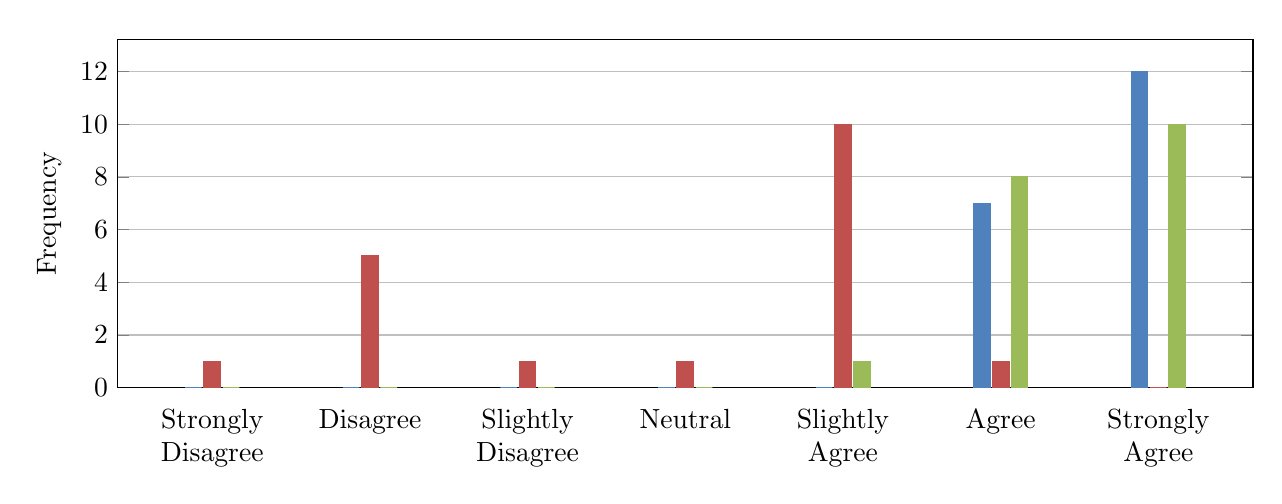
\begin{tikzpicture}
    \begin{axis}[
      width  = 16cm,
      height = 6cm,
      major x tick style = transparent,
      ybar=2*\pgflinewidth,
      bar width=6pt,
      ymajorgrids = true,
      ylabel = {Frequency},
      %xlabel = {Likert Scale Result},
      symbolic x coords= {-3,-2,-1,0,1,2,3},
      xticklabels = {Strongly Disagree,Disagree,Slightly Disagree,Neutral,Slightly Agree,Agree,Strongly Agree},
      xtick = data,
      ytick = {0,2,4,6,8,10,12,14},
      x tick label style  = {text width=2cm,align=center},
      scaled y ticks = false,
      % enlarge x limits=0.25,
      ymin=0,
      legend cell align=left,
      legend style={
              at={(1,1.05)},
              anchor=south east,
              column sep=1ex
      }
    ]
    \addplot[style={bblue,fill=bblue,mark=none}]
    	coordinates {(-3,0) (-2,0) (-1,0) (0,0) (1,0) (2,7) (3,12) };
    \addplot[style={rred,fill=rred,mark=none}]
    	coordinates {(-3,1) (-2,5) (-1,1) (0,1) (1,10) (2,1) (3,0) };
    \addplot[style={ggreen,fill=ggreen,mark=none}]
    	coordinates {(-3,0) (-2,0) (-1,0) (0,0) (1,1) (2,8) (3,10) };

    \end{axis}
\end{tikzpicture}

% \vspace{-20pt}
\paragraph{} Depending on its use, the inferred octave notation has the tradeoff that the octave is less easier inferred. There were no strong agreements and only one agreement that this was the case but the modal response was slight agreement. However many users didn't find this an issue and the distribution of responses is not significantly different to uniform. Overall this addition offered a significant improvement.

\subsection{Nested Instructions}

\begin{table}[!htbp]
\centering
% \caption{Grammar rules for turtle movement instructions. $z \in \mathbb{Z}, n \in \mathbb{N}, c \in \texttt{[A-Za-z]}^{+}$.}
\vspace{1pt}
\begin{tabular}{|l|l|l|} \hline
\textbf{Statement}&\textbf{Mode}&\textbf{p-value}\\ \hline
\mycbox{bblue} it is easier to parse the turtle instruction and tell &Agree&0.0003\\
what it will do.&& \\ \hline
\mycbox{rred} it is easier to repeat sections of notes.&Strongly Agree&0.0000\\ \hline
\mycbox{ggreen} Overall, system 2 is preferable.&Strongly Agree&0.0000\\ \hline
\end{tabular}
\label{evaluation:nestedInstructions}
\end{table}

\paragraph{} All participants found the addition of nested instructions with repeats preferable, with the majority strongly agreeing.

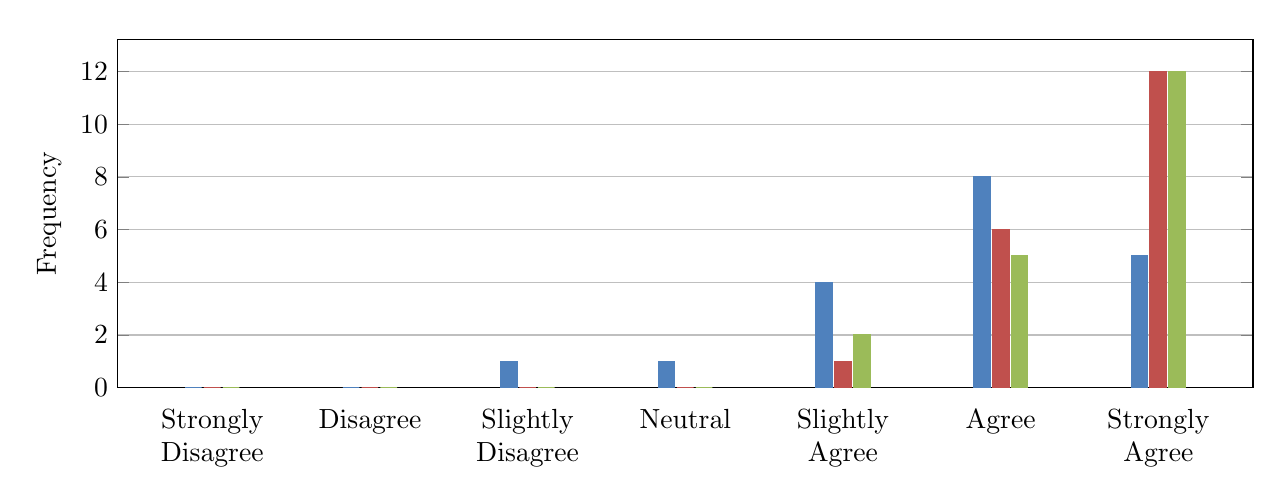
\begin{tikzpicture}
    \begin{axis}[
      % width  = \textwidth,
      width = 16cm,
      height = 6cm,
      major x tick style = transparent,
      ybar=2*\pgflinewidth,
      bar width=6pt,
      ymajorgrids = true,
      ylabel = {Frequency},
      %xlabel = {Likert Scale Result},
      symbolic x coords= {-3,-2,-1,0,1,2,3},
      xticklabels = {Strongly Disagree,Disagree,Slightly Disagree,Neutral,Slightly Agree,Agree,Strongly Agree},
      xtick = data,
      ytick = {0,2,4,6,8,10,12,14},
      x tick label style  = {text width=2cm,align=center},
      scaled y ticks = false,
      % enlarge x limits=0.25,
      ymin=0,
      legend cell align=left,
      legend style={
              at={(1,1.05)},
              anchor=south east,
              column sep=1ex
      }
    ]
    \addplot[style={bblue,fill=bblue,mark=none}]
    coordinates {(-3,0) (-2,0) (-1,1) (0,1) (1,4) (2,8) (3,5) };
    \addplot[style={rred,fill=rred,mark=none}]
    coordinates {(-3,0) (-2,0) (-1,0) (0,0) (1,1) (2,6) (3,12) };
    \addplot[style={ggreen,fill=ggreen,mark=none}]
    coordinates {(-3,0) (-2,0) (-1,0) (0,0) (1,2) (2,5) (3,12) };

        % \legend{It is easier to figure out the turtles path,It is easier to figure out what dynamics different notes are played at,It is easier to tell the order in which dynamics are applied,It is easier to write dynamics in the correct place,Overall system 2 is preferable}
    \end{axis}
\end{tikzpicture}

\subsection{Active Turtles List}

\begin{table}[!htbp]
\centering
% \caption{Grammar rules for turtle movement instructions. $z \in \mathbb{Z}, n \in \mathbb{N}, c \in \texttt{[A-Za-z]}^{+}$.}
\vspace{1pt}
\begin{tabular}{|l|l|l|} \hline
\textbf{Statement}&\textbf{Mode}&\textbf{p-value}\\ \hline
\mycbox{bblue} it is easier to tell if a certain turtle has been registered.&Strongly Agree&0.0000\\ \hline
\mycbox{rred} it is easier to see where the active turtles are.&(Strongly) Agree&0.0011\\ \hline
\mycbox{ggreen} it is easier to toggle the activation of turtles.in the&Agree&0.0038\\
correct place&& \\ \hline
\mycbox{ppurple} Overall, system 2 is preferable.&Strongly Agree&0.0000 \\ \hline
\end{tabular}
\label{evaluation:activeTurtles}
\end{table}

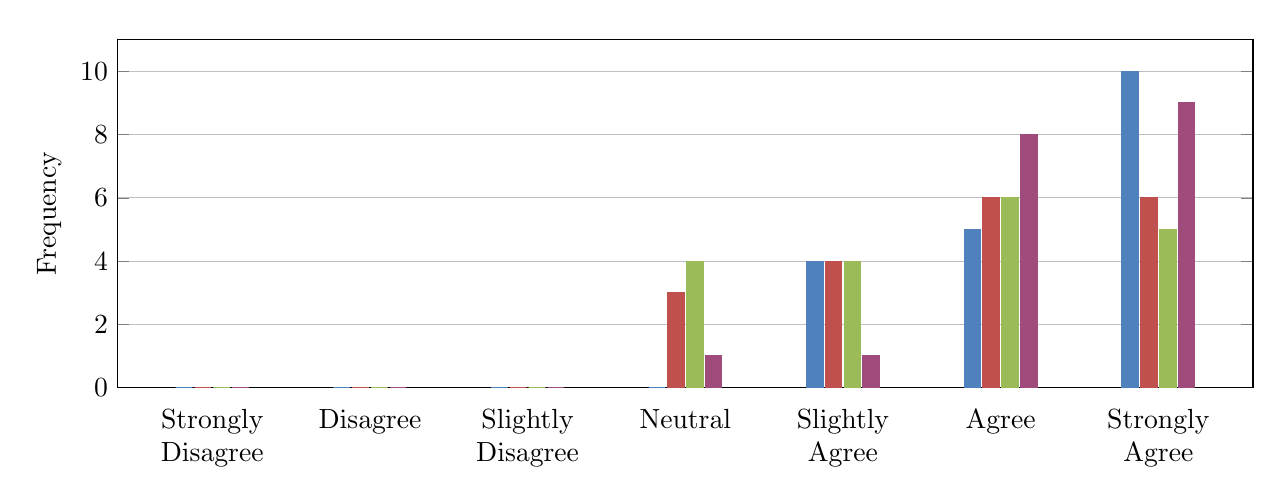
\begin{tikzpicture}
    \begin{axis}[
      % width  = \textwidth,
      width = 16cm,
      height = 6cm,
      major x tick style = transparent,
      ybar=2*\pgflinewidth,
      bar width=6pt,
      ymajorgrids = true,
      ylabel = {Frequency},
      %xlabel = {Likert Scale Result},
      symbolic x coords= {-3,-2,-1,0,1,2,3},
      xticklabels = {Strongly Disagree,Disagree,Slightly Disagree,Neutral,Slightly Agree,Agree,Strongly Agree},
      xtick = data,
      ytick = {0,2,4,6,8,10,12,14},
      x tick label style  = {text width=2cm,align=center},
      scaled y ticks = false,
      % enlarge x limits=0.25,
      ymin=0,
      legend cell align=left,
      legend style={
              at={(1,1.05)},
              anchor=south east,
              column sep=1ex
      }
    ]
    \addplot[style={bblue,fill=bblue,mark=none}]
    coordinates {(-3,0) (-2,0) (-1,0) (0,0) (1,4) (2,5) (3,10) };
    \addplot[style={rred,fill=rred,mark=none}]
    coordinates {(-3,0) (-2,0) (-1,0) (0,3) (1,4) (2,6) (3,6) };
    \addplot[style={ggreen,fill=ggreen,mark=none}]
    coordinates {(-3,0) (-2,0) (-1,0) (0,4) (1,4) (2,6) (3,5) };
    \addplot[style={ppurple,fill=ppurple,mark=none}]
    coordinates {(-3,0) (-2,0) (-1,0) (0,1) (1,1) (2,8) (3,9) };

        % \legend{It is easier to figure out the turtles path,It is easier to figure out what dynamics different notes are played at,It is easier to tell the order in which dynamics are applied,It is easier to write dynamics in the correct place,Overall system 2 is preferable}
    \end{axis}
\end{tikzpicture}

\paragraph{} The addition of a list of active turtles was found by all users to have a neutral or possitive effect on Excello.

\subsection{Continuous Volume}

\begin{table}[!htbp]
\centering
% \caption{Grammar rules for turtle movement instructions. $z \in \mathbb{Z}, n \in \mathbb{N}, c \in \texttt{[A-Za-z]}^{+}$.}
\vspace{1pt}
\begin{tabular}{|l|l|l|} \hline
\textbf{Statement}&\textbf{Mode}&\textbf{p-value}\\ \hline
\mycbox{bblue} it is more intuitive how loud a note will be played.&Disagree&0.6592\\
&Strongly Agree& \\ \hline
\mycbox{rred} the volumes available are less limited.&Strongly Agree&0.0000\\ \hline
\mycbox{ggreen} Overall, system 2 is preferable..&Agree&0.0003\\ \hline
\end{tabular}
\label{evaluation:continuousVolume}
\end{table}

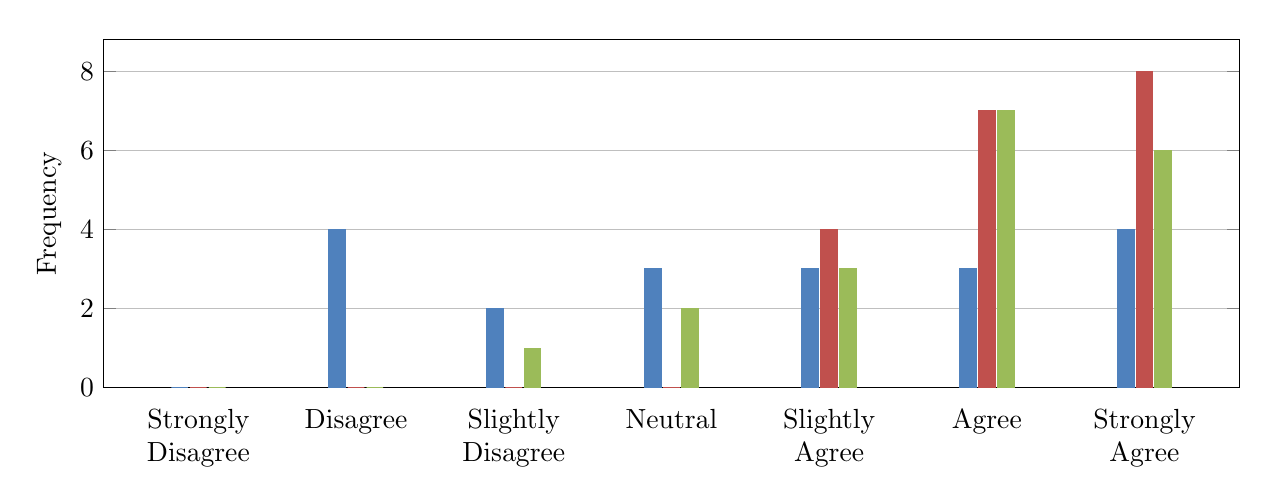
\begin{tikzpicture}
    \begin{axis}[
      % width  = \textwidth,
      width = 16cm,
      height = 6cm,
      major x tick style = transparent,
      ybar=2*\pgflinewidth,
      bar width=6pt,
      ymajorgrids = true,
      ylabel = {Frequency},
      %xlabel = {Likert Scale Result},
      symbolic x coords= {-3,-2,-1,0,1,2,3},
      xticklabels = {Strongly Disagree,Disagree,Slightly Disagree,Neutral,Slightly Agree,Agree,Strongly Agree},
      xtick = data,
      ytick = {0,2,4,6,8,10,12,14},
      x tick label style  = {text width=2cm,align=center},
      scaled y ticks = false,
      % enlarge x limits=0.25,
      ymin=0,
      legend cell align=left,
      legend style={
              at={(1,1.05)},
              anchor=south east,
              column sep=1ex
      }
    ]
    \addplot[style={bblue,fill=bblue,mark=none}]
    coordinates {(-3,0) (-2,4) (-1,2) (0,3) (1,3) (2,3) (3,4) };
    \addplot[style={rred,fill=rred,mark=none}]
    coordinates {(-3,0) (-2,0) (-1,0) (0,0) (1,4) (2,7) (3,8) };
    \addplot[style={ggreen,fill=ggreen,mark=none}]
    coordinates {(-3,0) (-2,0) (-1,1) (0,2) (1,3) (2,7) (3,6) };

        % \legend{It is easier to figure out the turtles path,It is easier to figure out what dynamics different notes are played at,It is easier to tell the order in which dynamics are applied,It is easier to write dynamics in the correct place,Overall system 2 is preferable}
    \end{axis}
\end{tikzpicture}

\paragraph{} There is no significant result for whether the ability to define volume in the range [0,1] is more intuitive. All users agreed that the volumes were less confined. However, only one user did not find this change preferable. Given that, it can be ommitted and the previous conventional dynamic markings used, this further supports the evidence that this addition was still successful.

\subsection{Automatic Stepping}

\begin{table}[!htbp]
\centering
% \caption{Grammar rules for turtle movement instructions. $z \in \mathbb{Z}, n \in \mathbb{N}, c \in \texttt{[A-Za-z]}^{+}$.}
\vspace{1pt}
\begin{tabular}{|l|l|l|} \hline
\textbf{Statement}&\textbf{Mode}&\textbf{p-value}\\ \hline
\mycbox{bblue} less mental work is required to write the turtle &Strongly Agree&0.0000\\
instructions.&& \\ \hline
\mycbox{rred} less work is required when more notes wish to be added.&Strongly Agree&0.0000\\ \hline
\mycbox{ggreen} Overall, system 2 is preferable.&Strongly Agree&0.0000\\ \hline
\end{tabular}
\label{evaluation:automaticStepping}
\end{table}

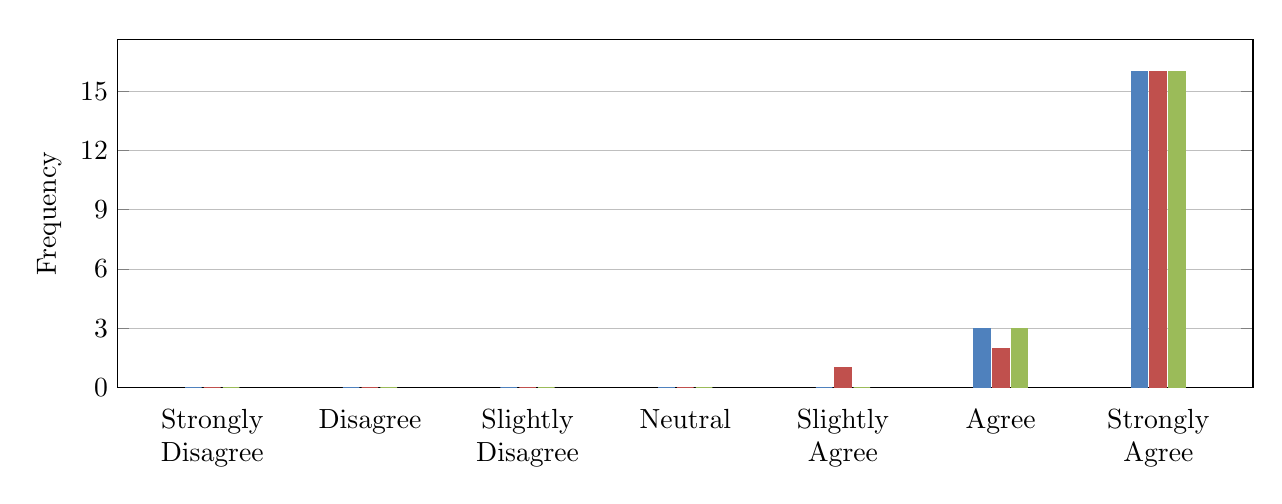
\begin{tikzpicture}
    \begin{axis}[
      % width  = \textwidth,
      width = 16cm,
      height = 6cm,
      major x tick style = transparent,
      ybar=2*\pgflinewidth,
      bar width=6pt,
      ymajorgrids = true,
      ylabel = {Frequency},
      %xlabel = {Likert Scale Result},
      symbolic x coords= {-3,-2,-1,0,1,2,3},
      xticklabels = {Strongly Disagree,Disagree,Slightly Disagree,Neutral,Slightly Agree,Agree,Strongly Agree},
      xtick = data,
      ytick = {0,3,6,9,12,15},
      x tick label style  = {text width=2cm,align=center},
      scaled y ticks = false,
      % enlarge x limits=0.25,
      ymin=0,
      legend cell align=left,
      legend style={
              at={(1,1.05)},
              anchor=south east,
              column sep=1ex
      }
    ]
    \addplot[style={bblue,fill=bblue,mark=none}]
    coordinates {(-3,0) (-2,0) (-1,0) (0,0) (1,0) (2,3) (3,16) };
    \addplot[style={rred,fill=rred,mark=none}]
    coordinates {(-3,0) (-2,0) (-1,0) (0,0) (1,1) (2,2) (3,16) };
    \addplot[style={ggreen,fill=ggreen,mark=none}]
    coordinates {(-3,0) (-2,0) (-1,0) (0,0) (1,0) (2,3) (3,16) };

        % \legend{It is easier to figure out the turtles path,It is easier to figure out what dynamics different notes are played at,It is easier to tell the order in which dynamics are applied,It is easier to write dynamics in the correct place,Overall system 2 is preferable}
    \end{axis}
\end{tikzpicture}

\paragraph{} The addition of this feature was particularly successful with 16 of the 19 users strongly agreeing the system was more preferable with automatic stepping available in the turtle instructions.

\subsection{Absolute Tempo}

\begin{table}[!htbp]
\centering
% \caption{Grammar rules for turtle movement instructions. $z \in \mathbb{Z}, n \in \mathbb{N}, c \in \texttt{[A-Za-z]}^{+}$.}
\vspace{1pt}
\begin{tabular}{|l|l|l|} \hline
\textbf{Statement}&\textbf{Mode}&\textbf{p-value}\\ \hline
\mycbox{bblue} it is easier to tell what the speed instruction&Strongly Agree&0.0000\\
 corresponds to&& \\ \hline
\mycbox{rred} giving an exact tempo (e.g. when transcribing sheet&Strongly Agree&0.0000\\
music) is easier&& \\ \hline
\mycbox{ggreen} Overall, system 2 is preferable.&Strongly Agree&0.0000\\ \hline
\end{tabular}
\label{evaluation:absoluteTempo}
\end{table}

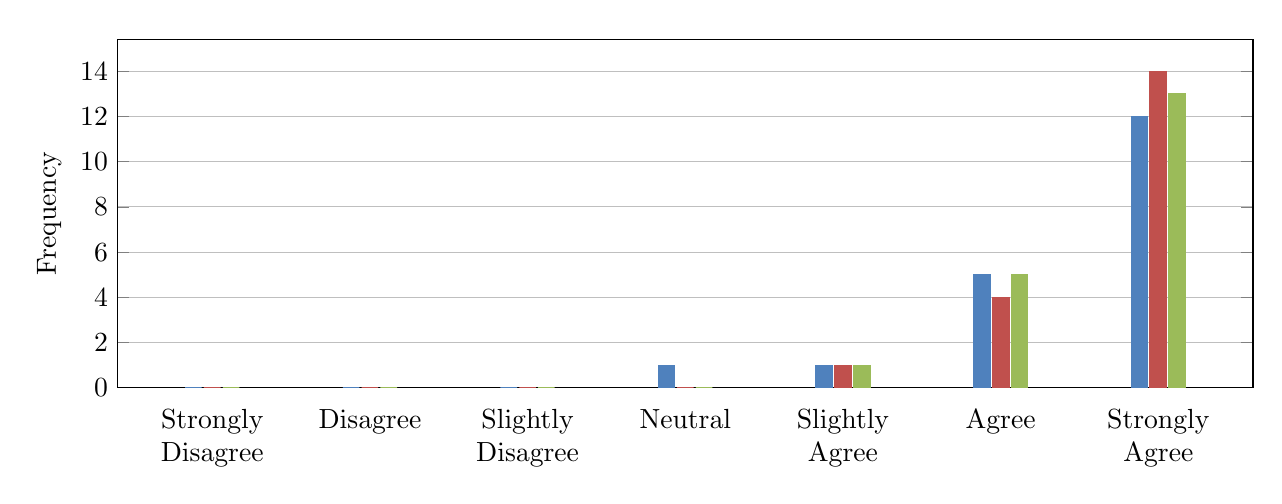
\begin{tikzpicture}
    \begin{axis}[
      % width  = \textwidth,
      width = 16cm,
      height = 6cm,
      major x tick style = transparent,
      ybar=2*\pgflinewidth,
      bar width=6pt,
      ymajorgrids = true,
      ylabel = {Frequency},
      %xlabel = {Likert Scale Result},
      symbolic x coords= {-3,-2,-1,0,1,2,3},
      xticklabels = {Strongly Disagree,Disagree,Slightly Disagree,Neutral,Slightly Agree,Agree,Strongly Agree},
      xtick = data,
      ytick = {0,2,4,6,8,10,12,14},
      x tick label style  = {text width=2cm,align=center},
      scaled y ticks = false,
      % enlarge x limits=0.25,
      ymin=0,
      legend cell align=left,
      legend style={
              at={(1,1.05)},
              anchor=south east,
              column sep=1ex
      }
    ]
    \addplot[style={bblue,fill=bblue,mark=none}]
    coordinates {(-3,0) (-2,0) (-1,0) (0,1) (1,1) (2,5) (3,12) };
    \addplot[style={rred,fill=rred,mark=none}]
    coordinates {(-3,0) (-2,0) (-1,0) (0,0) (1,1) (2,4) (3,14) };
    \addplot[style={ggreen,fill=ggreen,mark=none}]
    coordinates {(-3,0) (-2,0) (-1,0) (0,0) (1,1) (2,5) (3,13) };

        % \legend{It is easier to figure out the turtles path,It is easier to figure out what dynamics different notes are played at,It is easier to tell the order in which dynamics are applied,It is easier to write dynamics in the correct place,Overall system 2 is preferable}
    \end{axis}
\end{tikzpicture}

\paragraph{} The initial design was changed so that turtle speed was defined in absolute cells per minute. All users found this to be an improvement.

\paragraph{} Overall, the participatory design process was very successful. Multiple features were added to Excello to solve problems identified through formative evaluation sessions and longer-term feedback from users. There is signficant evidence to suggest all added features were found to improve Excello.

\section{Cognitive Dimensions of Notation}

\paragraph{} Figure \ref{fig:usage} shows the percentage of time users identified carrying out the different cognitive activities \cite{blackwell:tutorial} in Excello and in Sibelius. The Excello results are for 19 users with 12 users for Sibelius. Translation is a very important activity for both interfaces. Comparing the Excello results to Sibelius, there is more exploratory design but as users become more familiar with the system and the amount of existing Excello notation increases, modification and incrementation may become more important. Little time is spent searching for information in the notaiton in either.

\begin{figure}[ht]
\centering
\begin{subfigure}{.6\textwidth}
  \centering
    \begin{tikzpicture}
      \begin{axis}
        [
        height = 8cm,
        width = 7cm,
        ytick={1,2,3,4,5},
        yticklabels={Searching, Translation, Incrementation, Modification, Exploratory Design},
        xlabel = {Percentage of Time}
        ]
        \addplot+[
        	boxplot prepared={
        		median=10,
        		upper quartile=3.319672131,
        		lower quartile=10,
        		upper whisker=30,
        		lower whisker=0
        	},
        ] coordinates {};
        \addplot+[
        	boxplot prepared={
        		median=50,
        		upper quartile=45,
        		lower quartile=65,
        		upper whisker=100,
        		lower whisker=8
        	},
        ] coordinates {};
        \addplot+[
        	boxplot prepared={
        		median=10,
        		upper quartile=5,
        		lower quartile=15.69672131,
        		upper whisker=24,
        		lower whisker=0
        	},
        ] coordinates {};
        \addplot+[
        	boxplot prepared={
        		median=10,
        		upper quartile=5,
        		lower quartile=15.69672131,
        		upper whisker=30,
        		lower whisker=0
        	},
        ] coordinates {};
        \addplot+[
        	boxplot prepared={
        		median=10,
        		upper quartile=9,
        		lower quartile=27,
        		upper whisker=49,
        		lower whisker=0
        	},
        ] coordinates {};
      \end{axis}
    \end{tikzpicture}
  % \caption{A subfigure}
  \label{fig:sub1}
\end{subfigure}%
\begin{subfigure}{.4\textwidth}
  \centering
    \begin{tikzpicture}
      \begin{axis}
        [
        height = 8cm,
        width = 6.5cm,
        ytick={1,2,3,4,5},
        yticklabels={},
        xlabel = {Percentage of Time}
        ]
        \addplot+[
          boxplot prepared={
            median=10,
            upper quartile=5,
            lower quartile=11,
            upper whisker=27.27272727,
            lower whisker=0.460829493
          },
        ] coordinates {};
        \addplot+[
          boxplot prepared={
            median=40.22727273,
            upper quartile=30,
            lower quartile=50,
            upper whisker=60,
            lower whisker=13.82488479
          },
        ] coordinates {};
        \addplot+[
          boxplot prepared={
            median=20,
            upper quartile=15,
            lower quartile=29.25,
            upper whisker=41.47465438,
            lower whisker=4.545454545
          },
        ] coordinates {};
        \addplot+[
          boxplot prepared={
            median=16.09090909,
            upper quartile=10,
            lower quartile=30,
            upper whisker=41.47465438,
            lower whisker=5
          },
        ] coordinates {};
        \addplot+[
          boxplot prepared={
            median=9.166666667,
            upper quartile=4.886363636,
            lower quartile=15,
            upper whisker=20,
            lower whisker=0
          },
        ] coordinates {};
      \end{axis}
    \end{tikzpicture}
  % \caption{A subfigure}
  \label{fig:sub2}
\end{subfigure}
\caption{The percentage of time spent performing the different cognitive activites in Excello (left) and Sibelius (right).}
\label{fig:usage}
\end{figure}

\paragraph{} A series of statements assessing the CDN of the interface were selected \cite{blackwell:questionnaire}, these were assessed using a five-point (Strongly Disagree, Disagree, Neutral, Agree, Strongly Agree) Likert scale. To veryify the significance of the results, the data was combined into negative and non-negative categories and a chi-squared test performed. The questions asked, dimension being assessed, p-value from the chi-squared test and modal repsonse are shown in table \ref{evaluation:cdnTable}. The distribution of responses is shown in figure \ref{evaluation:cdnQuestions}.

\begin{table}[!htbp]
\centering
\vspace{1pt}
\begin{tabular}{|l|l|l|l|} \hline
\textbf{Statement}&\textbf{CDN}&\textbf{Mode}&\textbf{p-value}\\ \hline
\mycbox{bblue} (a) The notation used (In Excello: notes &Closeness&Agree&0.0004\\
/dynamics in cells and the definition of turtles)&of&& \\
is related to the result you are describing (In &Mapping&& \\
Excello: Musical output)&&& \\ \hline
\mycbox{rred} (b) Where there are different parts of the&Consistency&Agree&0.0087\\
notation that mean similar things, the&&& \\
similarity is clear from the way they appear. &&& \\ \hline
\mycbox{ggreen} (c) You can add extra marks (or colours or &Secondary&Agree&0.0020\\
format choices) to clarify, emphasise or repeat&Notation&& \\
what is there already. &&& \\ \hline
\mycbox{ppurple} (d) When you need to make changes to&Viscosity&Agree&0.0004 \\
previous, work it is easy to make the change.&&& \\ \hline
\mycbox{yyellow} (e) It is easy to see or find the various parts of &Visibility/&Agree&0.0087 \\
the notation while it is being created or changed.&Juxtaposition&& \\ \hline
\mycbox{bbrown} (f) If you need to compare or combine different&Visibility/&Agree&0.0312 \\
parts, you cansee them at the same time.&Juxtaposition&& \\ \hline
\end{tabular}
\caption{Questions and results for testing the CDN of Excello \label{evaluation:cdnTable}}
\end{table}

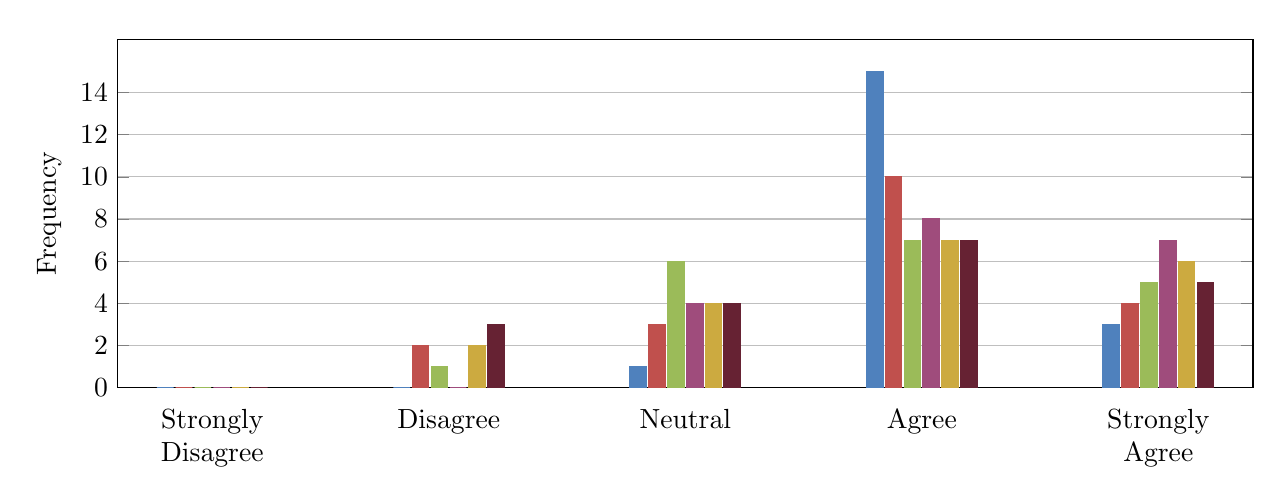
\begin{tikzpicture}
    \begin{axis}[
      % width  = \textwidth,
      width = 16cm,
      height = 6cm,
      major x tick style = transparent,
      ybar=2*\pgflinewidth,
      bar width=6pt,
      ymajorgrids = true,
      ylabel = {Frequency},
      %xlabel = {Likert Scale Result},
      symbolic x coords= {-3,-2,-1,0,1,2,3},
      xticklabels = {Strongly Disagree,Disagree,Neutral,Agree,Strongly Agree},
      xtick = data,
      ytick = {0,2,4,6,8,10,12,14},
      x tick label style  = {text width=2cm,align=center},
      scaled y ticks = false,
      % enlarge x limits=0.25,
      ymin=0,
      legend cell align=left,
      legend style={
              at={(1,1.05)},
              anchor=south east,
              column sep=1ex
      }
    ]
    \addplot[style={bblue,fill=bblue,mark=none}]
    	coordinates {(-3,0) (-2,0) (-1,1) (0,15) (1,3) };
    \addplot[style={rred,fill=rred,mark=none}]
    	coordinates {(-3,0) (-2,2) (-1,3) (0,10) (1,4) };
    \addplot[style={ggreen,fill=ggreen,mark=none}]
    	coordinates {(-3,0) (-2,1) (-1,6) (0,7) (1,5) };
    \addplot[style={ppurple,fill=ppurple,mark=none}]
    	coordinates {(-3,0) (-2,0) (-1,4) (0,8) (1,7) };
    \addplot[style={yyellow,fill=yyellow,mark=none}]
    	coordinates {(-3,0) (-2,2) (-1,4) (0,7) (1,6) };
    \addplot[style={bbrown,fill=bbrown,mark=none}]
    	coordinates {(-3,0) (-2,3) (-1,4) (0,7) (1,5) };

    \end{axis}
\end{tikzpicture}
\label{evaluation:cdnQuestions}

\paragraph{} As these questions were also answered for the user's interface of choice, a comparison to Sibelius can be made. As the data does not meet the assumptions of the t-test \cite{barry:likert}, I perofrmed a Wilcoxon matchd pairs signed-ranked test on the 12 pairs by encoding the five possible responses as -2,-1,0,1,2. For all six questions, there is no indication that the answers for the two interfaces come from populations with different means.

\subsection{Closeness of Mapping}

\paragraph{} Sibelius uses an established music notation as part of large professional software. As there is no significant evidence that the population means for Excello and Sibelius were different, this suggests Excello notation in spreadsheets has not compromised that closeness of mapping. This is helped by using an existing notation for defining the individual notes, the turtle instructions mapping to a movement through the grid, and by adjusting the speed argument to be an absolute, not relative, parameter. Being less familiar with staff notation, user 4 found the Sibelius's unintuitive.

\begin{figure}[tbh]
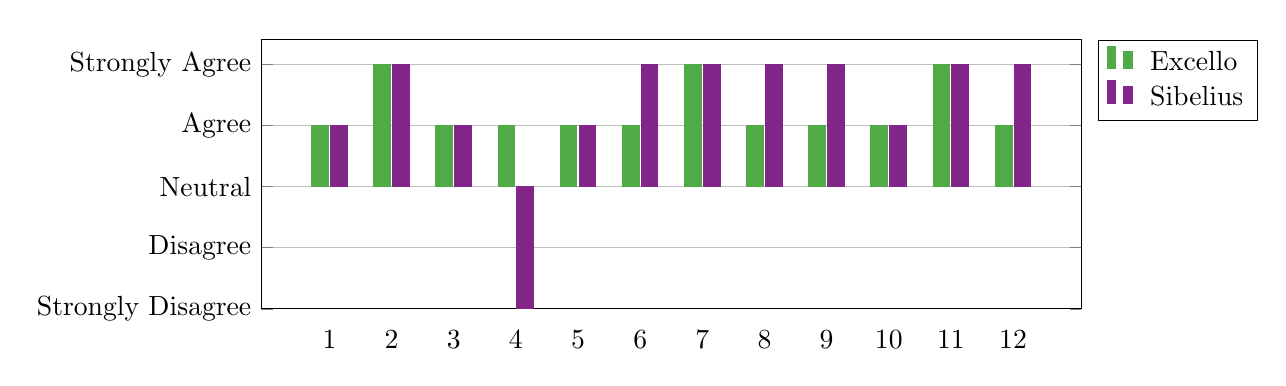
\begin{tikzpicture}
    \begin{axis}[
      % width  = \textwidth,
      width = 12cm,
      height = 5cm,
      major x tick style = transparent,
      ybar=2*\pgflinewidth,
      bar width=6pt,
      ymajorgrids = true,
      % ylabel = {Frequency},
      % %xlabel = {Likert Scale Result},
      % symbolic y coords= {-2,-1,0,1,2},
      yticklabels = {Strongly Disagree,Disagree,Neutral,Agree,Strongly Agree},
      xtick = {1,2,3,4,5,6,7,8,9,10,11,12},
      ytick = {-2,-1,0,1,2},
      ymin = -2,
      x tick label style  = {text width=2cm,align=center},
      scaled y ticks = false,
      % enlarge x limits=0.25,
      legend cell align=left,
      legend style={
              at={(1.02,1)},
              anchor=north west,
              column sep=1ex
      }
    ]
    \addplot[style={excelGreen,fill=excelGreen,mark=none}]
    	coordinates {(1,1) (2,2) (3,1) (4,1) (5,1) (6,1) (7,2) (8,1) (9,1) (10,1) (11,2) (12,1) };
    \addplot[style={sibPurple,fill=sibPurple,mark=none}]
    	coordinates {(1,1) (2,2) (3,1) (4,-2) (5,1) (6,2) (7,2) (8,2) (9,2) (10,1) (11,2) (12,2) };

    \legend{Excello,Sibelius}

    \end{axis}
\end{tikzpicture}
\caption{User responses for closeness of mapping for Excello and Sibelius from (a)}
\label{evaluation:clos}
\end{figure}

\subsection{Consistency}

\paragraph{} As each cell and turtle can only cause one note to play at a time, consistency is maintained by building up from these building blocks. Excello keeps consistency with the existing Excel interface by sharing notations (e.g. A1:A5 for ranges) and using the existing formula editor. Within the turtle instructions the ability to use a number after instructions for repeats holds for both individual instructions and sequences. This all helps contribute to there being no significant result from the Wilcoxon test.

\begin{figure}[tbh]
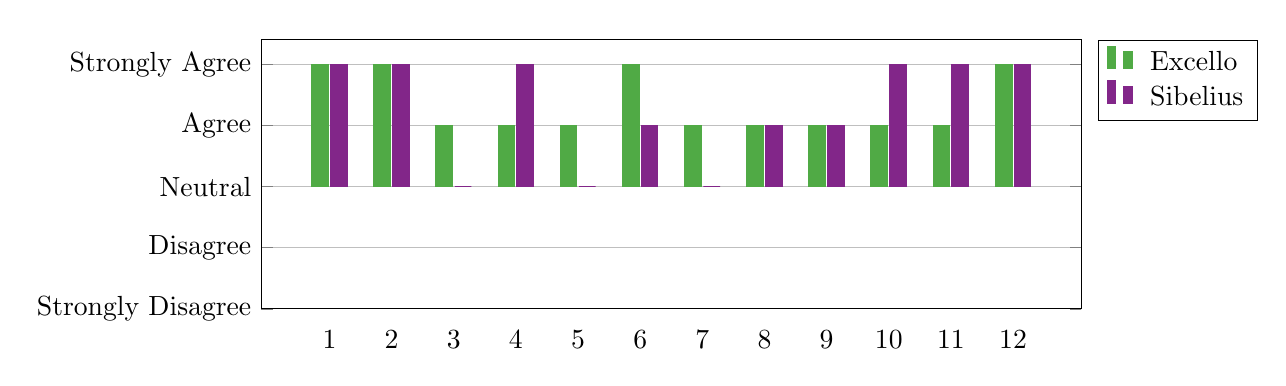
\begin{tikzpicture}
    \begin{axis}[
      % width  = \textwidth,
      width = 12cm,
      height = 5cm,
      major x tick style = transparent,
      ybar=2*\pgflinewidth,
      bar width=6pt,
      ymajorgrids = true,
      % ylabel = {Frequency},
      % %xlabel = {Likert Scale Result},
      % symbolic y coords= {-2,-1,0,1,2},
      yticklabels = {Strongly Disagree,Disagree,Neutral,Agree,Strongly Agree},
      xtick = {1,2,3,4,5,6,7,8,9,10,11,12},
      ytick = {-2,-1,0,1,2},
      ymin = -2,
      x tick label style  = {text width=2cm,align=center},
      scaled y ticks = false,
      % enlarge x limits=0.25,
      legend cell align=left,
      legend style={
              at={(1.02,1)},
              anchor=north west,
              column sep=1ex
      }
    ]

    \addplot[style={excelGreen,fill=excelGreen,mark=none}]
    	coordinates {(1,2) (2,2) (3,1) (4,1) (5,1) (6,2) (7,1) (8,1) (9,1) (10,1) (11,1) (12,2) };
    \addplot[style={sibPurple,fill=sibPurple,mark=none}]
    	coordinates {(1,2) (2,2) (3,0) (4,2) (5,0) (6,1) (7,0) (8,1) (9,1) (10,2) (11,2) (12,2) };

    \legend{Excello,Sibelius}

    \end{axis}
\end{tikzpicture}
\caption{User responses for consistency for Excello and Sibelius from (b)}
\label{evaluation:cons}
\end{figure}

\subsection{Secondary Notation}

\paragraph{} Given the time spent performing translation, secondary notation is particularly important \cite{blackwell:notation}. Given that Excello abstracts time from the axes of the grid the distribution of parts is up to the user and cells can be used for arbitrary marks. As a result the existing features of Excel to format and group cells is already available. This is alredy utilised by the highlighting of notes and turtles. That there is no significant difference in population means, this suggests that the spreadsheet paradigm can provide an equal secondary notaion abilities to Sibelius, software already equipped with numerous ways to customise a score.

\begin{figure}[tbh]
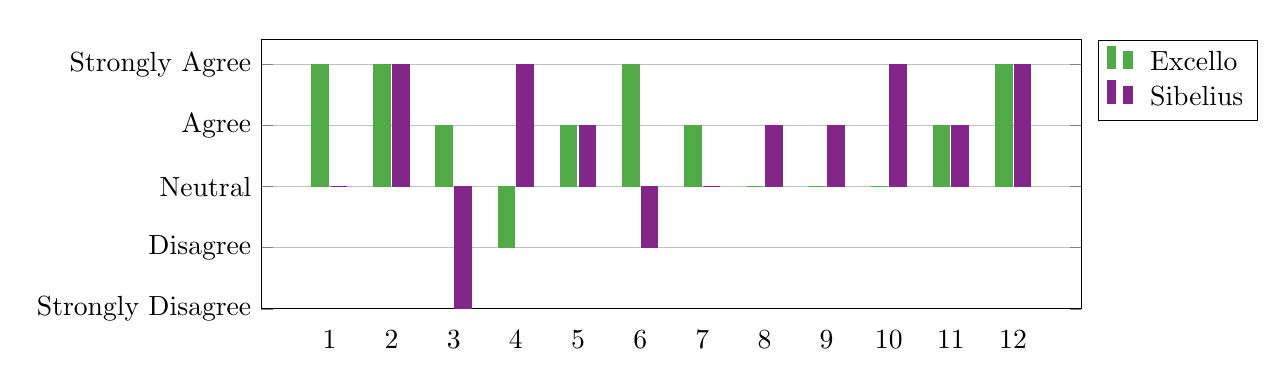
\begin{tikzpicture}
    \begin{axis}[
      % width  = \textwidth,
      width = 12cm,
      height = 5cm,
      major x tick style = transparent,
      ybar=2*\pgflinewidth,
      bar width=6pt,
      ymajorgrids = true,
      % ylabel = {Frequency},
      % %xlabel = {Likert Scale Result},
      % symbolic y coords= {-2,-1,0,1,2},
      yticklabels = {Strongly Disagree,Disagree,Neutral,Agree,Strongly Agree},
      xtick = {1,2,3,4,5,6,7,8,9,10,11,12},
      ytick = {-2,-1,0,1,2},
      ymin = -2,
      x tick label style  = {text width=2cm,align=center},
      scaled y ticks = false,
      % enlarge x limits=0.25,
      legend cell align=left,
      legend style={
              at={(1.02,1)},
              anchor=north west,
              column sep=1ex
      }
    ]

    \addplot[style={excelGreen,fill=excelGreen,mark=none}]
      coordinates {(1,2) (2,2) (3,1) (4,-1) (5,1) (6,2) (7,1) (8,0) (9,0) (10,0) (11,1) (12,2) };
    \addplot[style={sibPurple,fill=sibPurple,mark=none}]
      coordinates {(1,0) (2,2) (3,-2) (4,2) (5,1) (6,-1) (7,0) (8,1) (9,1) (10,2) (11,1) (12,2) };

    \legend{Excello,Sibelius}

    \end{axis}
\end{tikzpicture}
\caption{User responses for secondary notation for Excello and Sibelius from (c)}
\label{evaluation:secn}
\end{figure}

\subsection{Viscosity}

\paragraph{} By allowing dynamics and octave marking to be ommitted and the ability for turtles to step forward automatically, there is low resistance to making additions and changes to the music. The button to toggle turtle activations dramatically reduces the actions required to turn turtles on and off. Furthermore Excel allows for the easy editing and movement of cells. No significant result in the Wilcoxon test suggests the interfaces have comparable viscosity.

\begin{figure}[tbh]
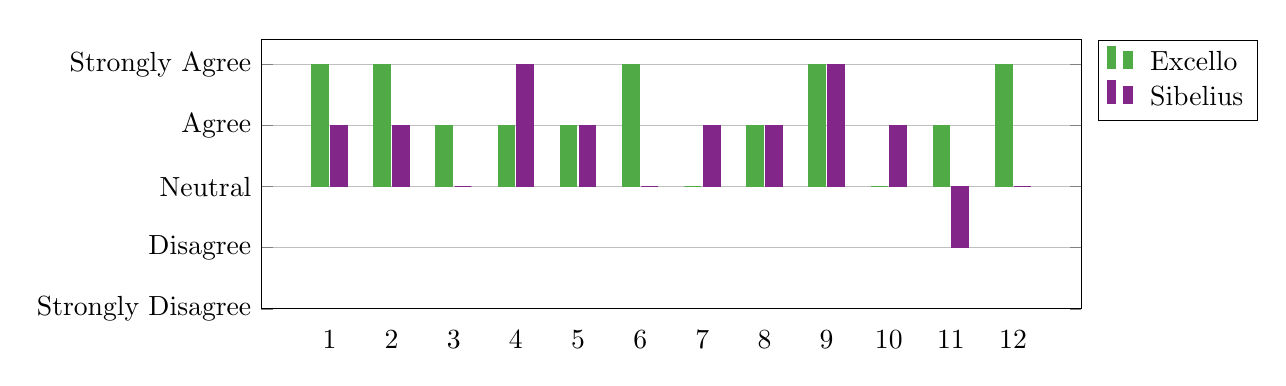
\begin{tikzpicture}
    \begin{axis}[
      % width  = \textwidth,
      width = 12cm,
      height = 5cm,
      major x tick style = transparent,
      ybar=2*\pgflinewidth,
      bar width=6pt,
      ymajorgrids = true,
      % ylabel = {Frequency},
      % %xlabel = {Likert Scale Result},
      % symbolic y coords= {-2,-1,0,1,2},
      yticklabels = {Strongly Disagree,Disagree,Neutral,Agree,Strongly Agree},
      xtick = {1,2,3,4,5,6,7,8,9,10,11,12},
      ytick = {-2,-1,0,1,2},
      ymin = -2,
      x tick label style  = {text width=2cm,align=center},
      scaled y ticks = false,
      % enlarge x limits=0.25,
      legend cell align=left,
      legend style={
              at={(1.02,1)},
              anchor=north west,
              column sep=1ex
      }
    ]

    \addplot[style={excelGreen,fill=excelGreen,mark=none}]
    	coordinates {(1,2) (2,2) (3,1) (4,1) (5,1) (6,2) (7,0) (8,1) (9,2) (10,0) (11,1) (12,2) };
    \addplot[style={sibPurple,fill=sibPurple,mark=none}]
    	coordinates {(1,1) (2,1) (3,0) (4,2) (5,1) (6,0) (7,1) (8,1) (9,2) (10,1) (11,-1) (12,0) };

    \legend{Excello,Sibelius}

    \end{axis}
\end{tikzpicture}
\caption{User responses for viscosity for Excello and Sibelius from (d)}
\label{evaluation:visc}
\end{figure}

\subsection{Visability / Juxtaposition}

\paragraph{} For both questions there was no significant difference in population mean. This suggests that the This suggests that the speadsheet interface can provide a similar abilty to view components than Sibelius.

\begin{figure}[tbh]
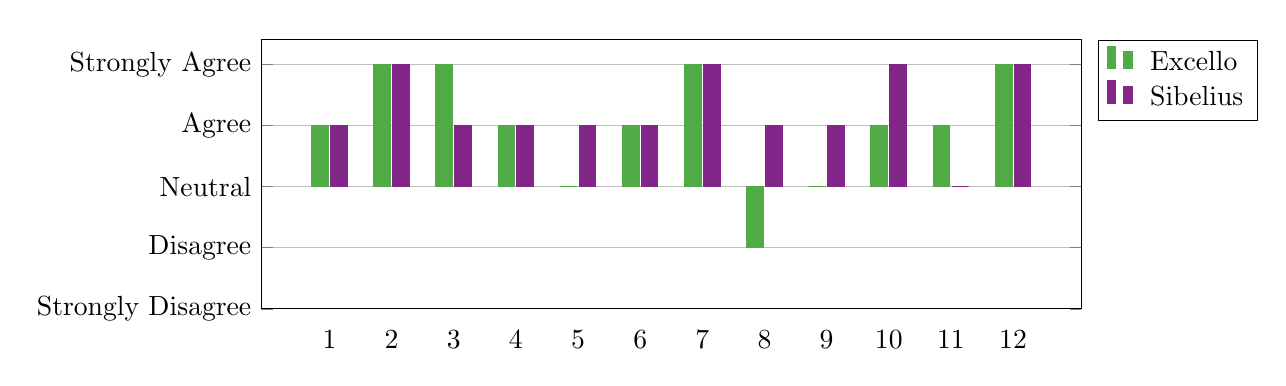
\begin{tikzpicture}
    \begin{axis}[
      % width  = \textwidth,
      width = 12cm,
      height = 5cm,
      major x tick style = transparent,
      ybar=2*\pgflinewidth,
      bar width=6pt,
      ymajorgrids = true,
      % ylabel = {Frequency},
      % %xlabel = {Likert Scale Result},
      % symbolic y coords= {-2,-1,0,1,2},
      yticklabels = {Strongly Disagree,Disagree,Neutral,Agree,Strongly Agree},
      xtick = {1,2,3,4,5,6,7,8,9,10,11,12},
      ytick = {-2,-1,0,1,2},
      ymin = -2,
      x tick label style  = {text width=2cm,align=center},
      scaled y ticks = false,
      % enlarge x limits=0.25,
      legend cell align=left,
      legend style={
              at={(1.02,1)},
              anchor=north west,
              column sep=1ex
      }
    ]

    \addplot[style={excelGreen,fill=excelGreen,mark=none}]
    	coordinates {(1,1) (2,2) (3,2) (4,1) (5,0) (6,1) (7,2) (8,-1) (9,0) (10,1) (11,1) (12,2) };
    \addplot[style={sibPurple,fill=sibPurple,mark=none}]
    	coordinates {(1,1) (2,2) (3,1) (4,1) (5,1) (6,1) (7,2) (8,1) (9,1) (10,2) (11,0) (12,2) };

    \legend{Excello,Sibelius}

    \end{axis}
\end{tikzpicture}
\caption{User responses for visibility/juxtaposition for Excello and Sibelius from (e)}
\label{evaluation:viju1}
\end{figure}

\begin{figure}[tbh]
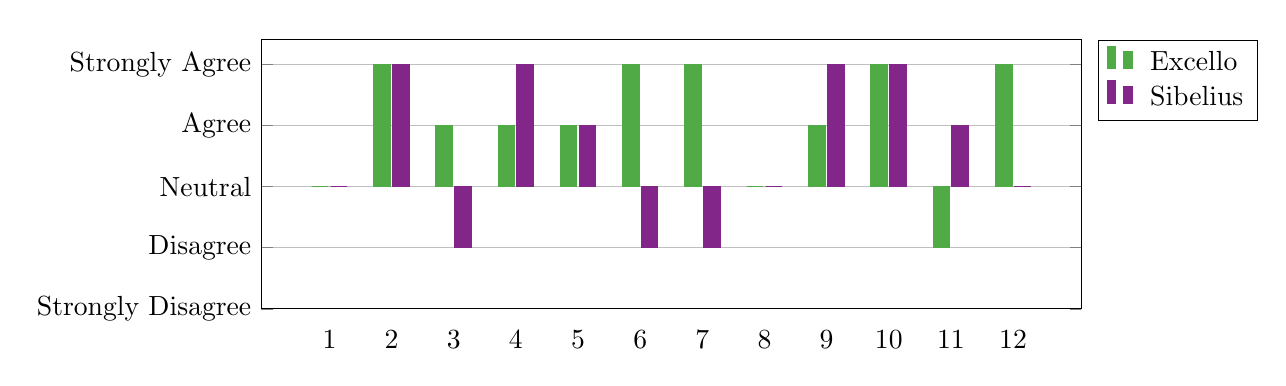
\begin{tikzpicture}
    \begin{axis}[
      % width  = \textwidth,
      width = 12cm,
      height = 5cm,
      major x tick style = transparent,
      ybar=2*\pgflinewidth,
      bar width=6pt,
      ymajorgrids = true,
      % ylabel = {Frequency},
      % %xlabel = {Likert Scale Result},
      % symbolic y coords= {-2,-1,0,1,2},
      yticklabels = {Strongly Disagree,Disagree,Neutral,Agree,Strongly Agree},
      xtick = {1,2,3,4,5,6,7,8,9,10,11,12},
      ytick = {-2,-1,0,1,2},
      ymin = -2,
      x tick label style  = {text width=2cm,align=center},
      scaled y ticks = false,
      % enlarge x limits=0.25,
      legend cell align=left,
      legend style={
              at={(1.02,1)},
              anchor=north west,
              column sep=1ex
      }
    ]

    \addplot[style={excelGreen,fill=excelGreen,mark=none}]
    	coordinates {(1,0) (2,2) (3,1) (4,1) (5,1) (6,2) (7,2) (8,0) (9,1) (10,2) (11,-1) (12,2) };
    \addplot[style={sibPurple,fill=sibPurple,mark=none}]
    	coordinates {(1,0) (2,2) (3,-1) (4,2) (5,1) (6,-1) (7,-1) (8,0) (9,2) (10,2) (11,1) (12,0) };

    \legend{Excello,Sibelius}

    \end{axis}
\end{tikzpicture}
\caption{User responses for visibility/juxtaposition for Excello and Sibelius from (f)}
\label{evaluation:viju2}
\end{figure}

\paragraph{} Whilst there was no significant evidence to suggest Excello outperformed Sibelius across these CDN, that it achieved similar results to Sibelius, an established music notation editing package, suggests that Excello is successful interface for writing music.

\subsection{Other Dimensions}

\paragraph{} If users are unfamiliar with the turtle paradigm, this may reduce the \textit{role-expressiveness}. Turtles and notes are the only components of the spreadsheet and these are identified by highlighting.Whilst the Excel is very flexible and notes and turtles can be added in any order, adding an additional part may required many line insertions which increases the \textit{premature committment}. The dual-formalism of the turtles and notes could create high \textit{diffuseness} but the freedom of the user to lay these out allows this to be minimized as in figure \ref{evaluation:excelloFranzRedacted}. This also shows how representations can have goot \textit{synopsie}, as the notes or turtles don't need to be examined to understand what is happening. However, this may come at the expense of \textit{hidden dependencies} where it is not immediately clear which notes are triggered by which turtles. Volume is also dependent on the notes turtles play before it. But as a single cell could be played at multiple volumes, this is a tradeoff of this design decission.

\paragraph{} As well as the \texttt{m*} notation decreasing \textit{viscosity}, it also improves the \textit{progressive evaluation} as turtles can be played before a whole part has been transcribed. The highlighting of cells also helps users receive more feedback. The ability to define a turtle and fill in the notes later also improves the \textit{provisionality}. The use of \texttt{m*} also reduce the \textit{hard mental operations} required. The chord input tool also removes the need to calculate the notes of a chord.

\paragraph{} Spreadsheets are "an abstraction-hating system" \cite{blackwell:tutorial}, therefore little \textit{abstraction} is provided by Excel, but the grouping of turtles in one definition and nested bracketing in turtle movement instructions improve this. These features also provide good \textit{legibility}.

\section{Ethics and Data Handling}

\paragraph{} After ethics approval, the pilot session for the formative evaluation session was designed. Participants were provided with a consent form explaining the project and the format of the session. Participants had the choice to remain annonymous so they would not appear in acknowledgements, if so, all their data was labelled with a unique ID for participants to be able to use to request removal or anonymising of their data. All participant data was only seen by myself. Sessions were audio recorded with recordings types up after the session and then deleted. All participant data was also backed up on GitHub with the rest of the project but in an encrypted folder. After the pilot session (also performed for summative evaluation), the session was revised before continuing with the remaining sessions.
